Finding the system of equations to solve to find consistent initial conditions and using the dummy derivatives method to reduce the index to 1. 

The system:
\begin{align*}
	\dot x &= u & e_1\\
	\dot y &= v & e_2\\
	m\,\dot u &= x\,\lambda & e_3\\
	m\,\dot v &= y\,\lambda - m\,g & e_4\\
	0 &= x^2 + y^2 - l^2 & e_5
\end{align*}

Pantelides gives (1,1,0,0,2), i.e:
\begin{align*}
	\ddot x &= \dot u & \dot e_1\\
	\ddot y &= \dot v & \dot e_2\\
	m\,\dot u &= x\,\lambda & e_3\\
	m\,\dot v &= y\,\lambda - m\,g & e_4\\
	0 &= u^2 + v^2 + x\,\ddot x + y\,\ddot y & \ddot e_5
\end{align*}
$\mathcal{G} = (\ddot x,\ddot y,\dot u,\dot v, \lambda)$ can be written as follows:
\begin{align*}
	\begin{tabular}{c|c c c c c}
		& $\ddot x$ & $\ddot y$ & $\dot u$ & $\dot v$ & $\lambda$ \\
		\hline
		$\dot e_1$ & 1 & & 1 & &\\
		$\dot e_2$ & & 1 & & 1 &\\
		$e_3$ & & & $m$ & & $x$\\
		$e_4$ & & & & $m$ & $y$\\
		$\ddot e_5$ & $x$ & $y$ & & &\\	
	\end{tabular} & & \implies & \begin{tabular}{c|c c c c c}
	 & $\ddot x$ & $\ddot y$ & $\dot u$ & $\dot v$ & $\lambda$ \\
	\hline
	$\dot e_1$ & 1 & & 1 & &\\
	$\dot e_2$ & & 1 & & 1 &\\
	$\ddot e_5$ & $x$ & $y$ & & &\\		
\end{tabular}
\end{align*}

\fbox{\begin{minipage}[h!]{\textwidth}
	Assuming $x \neq 0$ then ($\ddot x,\dot u,\dot v$) are chosen as dummy variables. However, $x = 0$ is an equilibrium point of the system. Therefore, ($\ddot y,\dot u,\dot v$) are the chosen dummy variables with the assumption $y \neq 0$. 
\end{minipage}}	

one more dummy variable is required. Therefore, the following equations are considered :
\begin{align*}
	\dot x &= u & e_1\\
	\dot y &= v & e_2\\
	0 &= x\,\dot x + y\,\dot y & \dot e_5
\end{align*}
$\mathcal{G} = (\dot x,\dot y, u)$ can be written as follows:
\begin{align*}
	\begin{tabular}{c|c c c c c}
		& $\dot x$ & $\dot y$ & $ u$ & $ v$ & $\lambda$ \\
		\hline
		$e_1$ & 1 & & 1 & &\\
		$e_2$ & & 1 & & 1 &\\
		$\dot e_5$ & $x$ & $y$ & & &\\		
	\end{tabular} & & \implies & \begin{tabular}{c|c c c c c}
		& $\dot x$ & $\dot y$ & $u$ & $v$ & $\lambda$ \\
		\hline
		$\dot e_5$ & $x$ & $y$ & & &\\		
	\end{tabular}
\end{align*}
\fbox{\begin{minipage}[h!]{\textwidth}
	Since $y \neq 0$ is the assumption, ($\dot  y$) is chosen as the dummy variable. 
\end{minipage}}	
%\begin{description}
%	\item[Assumption 2] Considering $y \neq 0$. 
%\end{description}
%Therefore, we can choose $\dot x$ or $\dot y$ as the dummy variable. $\dot x$ was chosen. \\
%\fbox{\begin{minipage}[h!]{\textwidth}
%	\textbf{Note:} Choosing $\dot x$ would result in a singular matrix when $x = 0$. This is a problem since $x = 0$ is an equilibrium point and the pendulum always passes through this point. 
%\end{minipage}}	

The dummy variables are ($y',y'',u',v'$). 

The equation set with variables $(x,y,y',y'',u,v,u',v',\lambda)$ is given as follows:
\begin{align*}
	\dot x &= u & e_1\\
	\dot u &= u' & \dot e_1\\
	y' &= v & e_2\\
	y'' &= v' & \dot e_2\\
	m\,u' &= x\,\lambda & e_3\\
	m\,v' &= y\,\lambda - m\,g & e_4\\
	0 &= x^2 + y^2 - l^2 & e_5\\
	0 &= x\,u'+ y\,y' & \dot e_5 \\
	0 &= u^2 + v^2 + x\,u' + y\,y'' & \ddot e_5
\end{align*}
The simulation results are presented in the following figure:\\
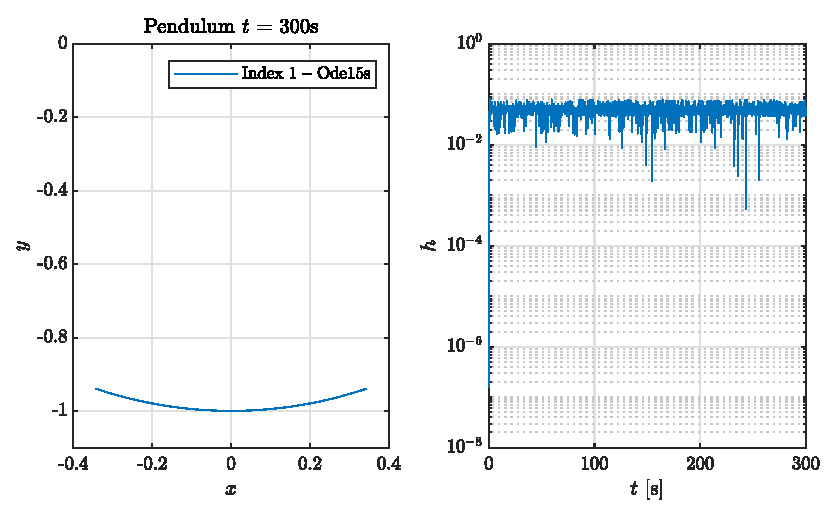
\includegraphics[width=0.9\textwidth]{Figures/Ugf2_30.eps}

The code is as follows:
\begin{lstlisting}
	clear all; clc; 
	% the DAE system for the pendulum
	% parameters
	m = 2.6; % mass of the pendulam
	g = 9.8; 
	l = 1; % length of the pendulam
	
	% The Model
	% y(1) = x
	% y(2) = u
	% y(3) = y'
	% y(4) = y''
	% y(5) = y
	% y(6) = v
	% y(7) = u'
	% y(8) = v'
	% y(9) = lambda
	pendulam_idx1 = @(t,y) [ ...
	y(2);...
	y(7);...
	y(6) - y(3);...
	y(8) - y(4);...
	y(1)*y(9) - m*y(7);...
	y(5)*y(9) - m*g - m*y(8);...
	y(1)^2 + y(5)^2 - l^2;...
	- y(5)*y(3);...
	y(2)^2 + y(6)^2 + y(1)*y(7) + y(5)*y(4)]; 
	% simulation 
	tsim_l = [0 300]; % long simulation time
	
	M_idx1 = zeros(9,9); % mass matrix
	M_idx1(1,1) = 1; M_idx1(2,2) = 1; 
	options_idx1 = odeset('Mass',M_idx1); 
	
	y0 = -l; y0_idx0 = [0;1;0;0;y0;0;0;0;0]; % initial conditions
	
	[t_idx1_l,y_idx1_l] = ode15s(@(t,y) pendulam_idx1(t,y),tsim_l,...
	y0_idx0,options_idx1);
	
	% Plots
	figure(1)
	clf
	
	subplot(121)
	plot(t_idx1_l(:,1),y_idx1_l(:,5)) %,y_idx0_s(:,1),y_idx0_s(:,2),'--')
	grid on; legend('Index 1 -- Ode15s') %,'Index 0 -- Ode45')
	ax(1) = figtex(gca,1);
	xlabel('$x$'); ylabel('$y$'); title('Pendulum $t$ = 300s');
	ylim([-l*1.1 0])
	
	subplot(122)
	semilogy(t_idx1_l(2:end),diff(t_idx1_l)) %,t_idx0_s(2:end),diff(t_idx0_s),'--')
	grid on; ax(3) = figtex(gca);
	xlabel('$t$ [s]'); ylabel('$h$');
	
	figsize(1,0.35);
	saveas(gcf,'Figures/Ugf2_30','epsc');		
\end{lstlisting}